\begin{wrapfigure}[0]{r}[0cm]{6cm}
	\vspace{-4cm}
  	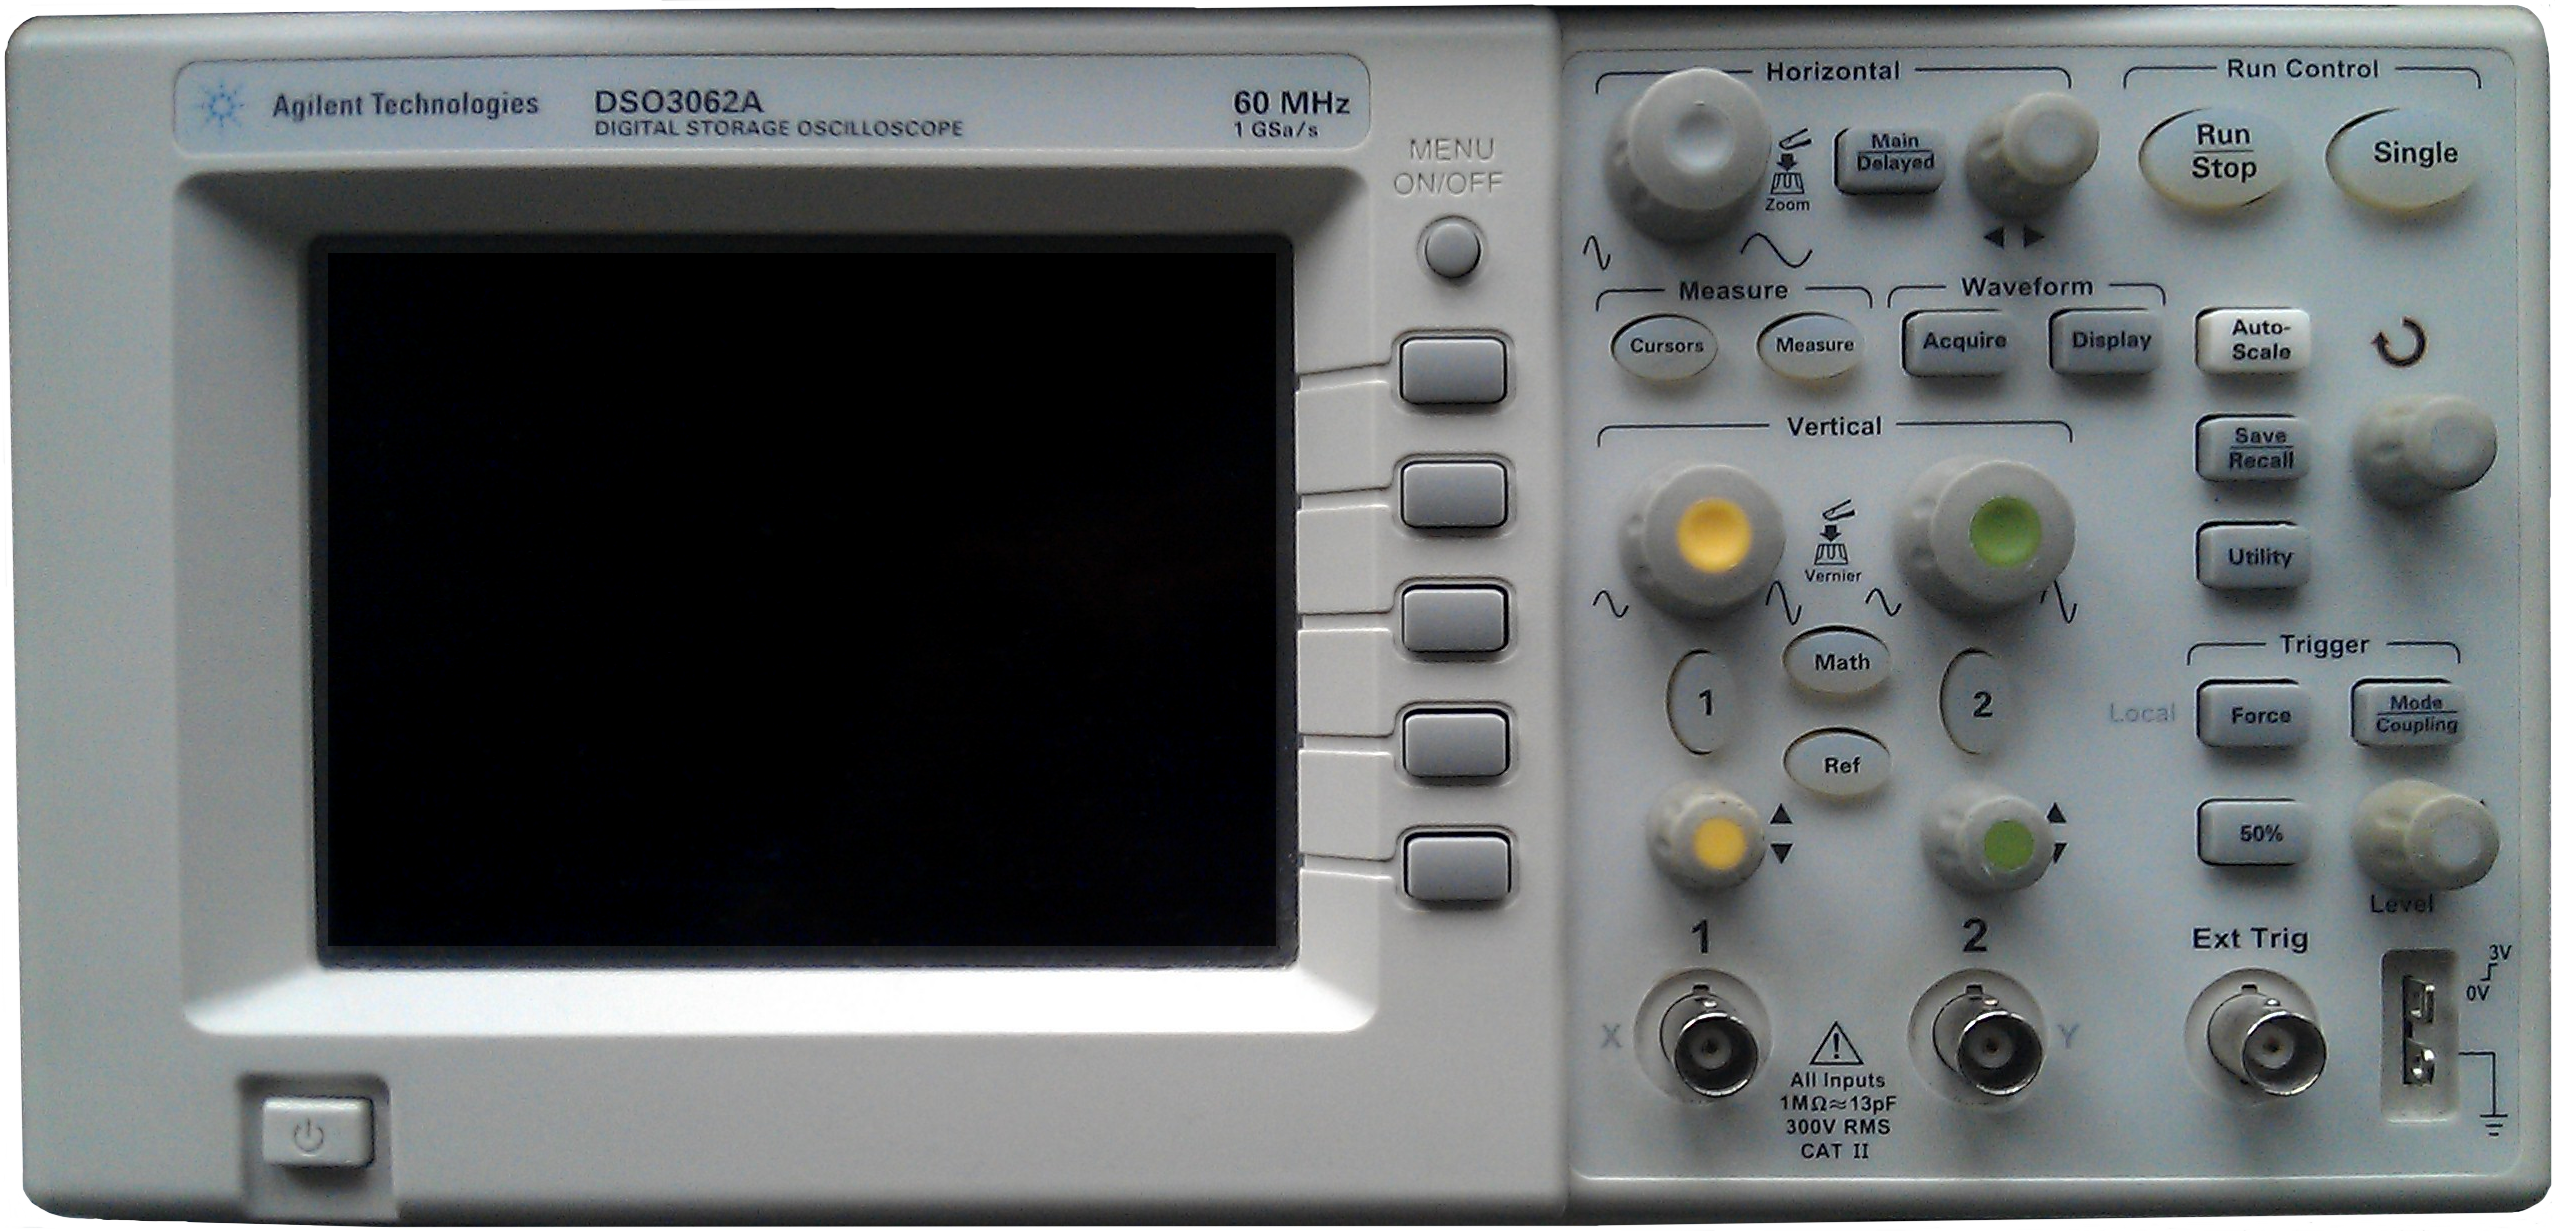
\includegraphics[scale=0.08]{Oszi/Bilder/oszi_foto.png}
 	\vspace{-4cm}
	\end{wrapfigure}

\section*{Theorie}

Mit Hilfe eines Oszilloskops lassen sich die zeitlichen Verläufe einer Messgröße darstellen. In erster Linie wird die Spannung in Abhängigkeit von der Zeit dargestellt.
Grundsätzlich muss darauf geachtet werden, dass nur Spannungen gegen Masse gemessen werden können.
Es kann sein, dass das Gehäuse des Oszilloskops mit dem Schutzleiter des Versorgungsnetzes verbunden ist, daher kann es notwendig sein, Messobjekte über einen Trenntrafo zu betreiben.\par

Der eingestellte Spannungs- und Zeitbereich am Oszilloskop (siehe Abbildung \ref{Anzeige_Oszi} \textit{Kanal 1 - Status}) verhält sich pro div.
Das ist die  Abkürzung für divit (Teil) und bezieht sich auf die Rastereinheit des Bildschirms. In Abbildung \ref{Anzeige_Oszi} sind dies also $20mV$ bzw. $500\mu s$ pro Rastereinheit.\par

\begin{figure}[H]
\centering
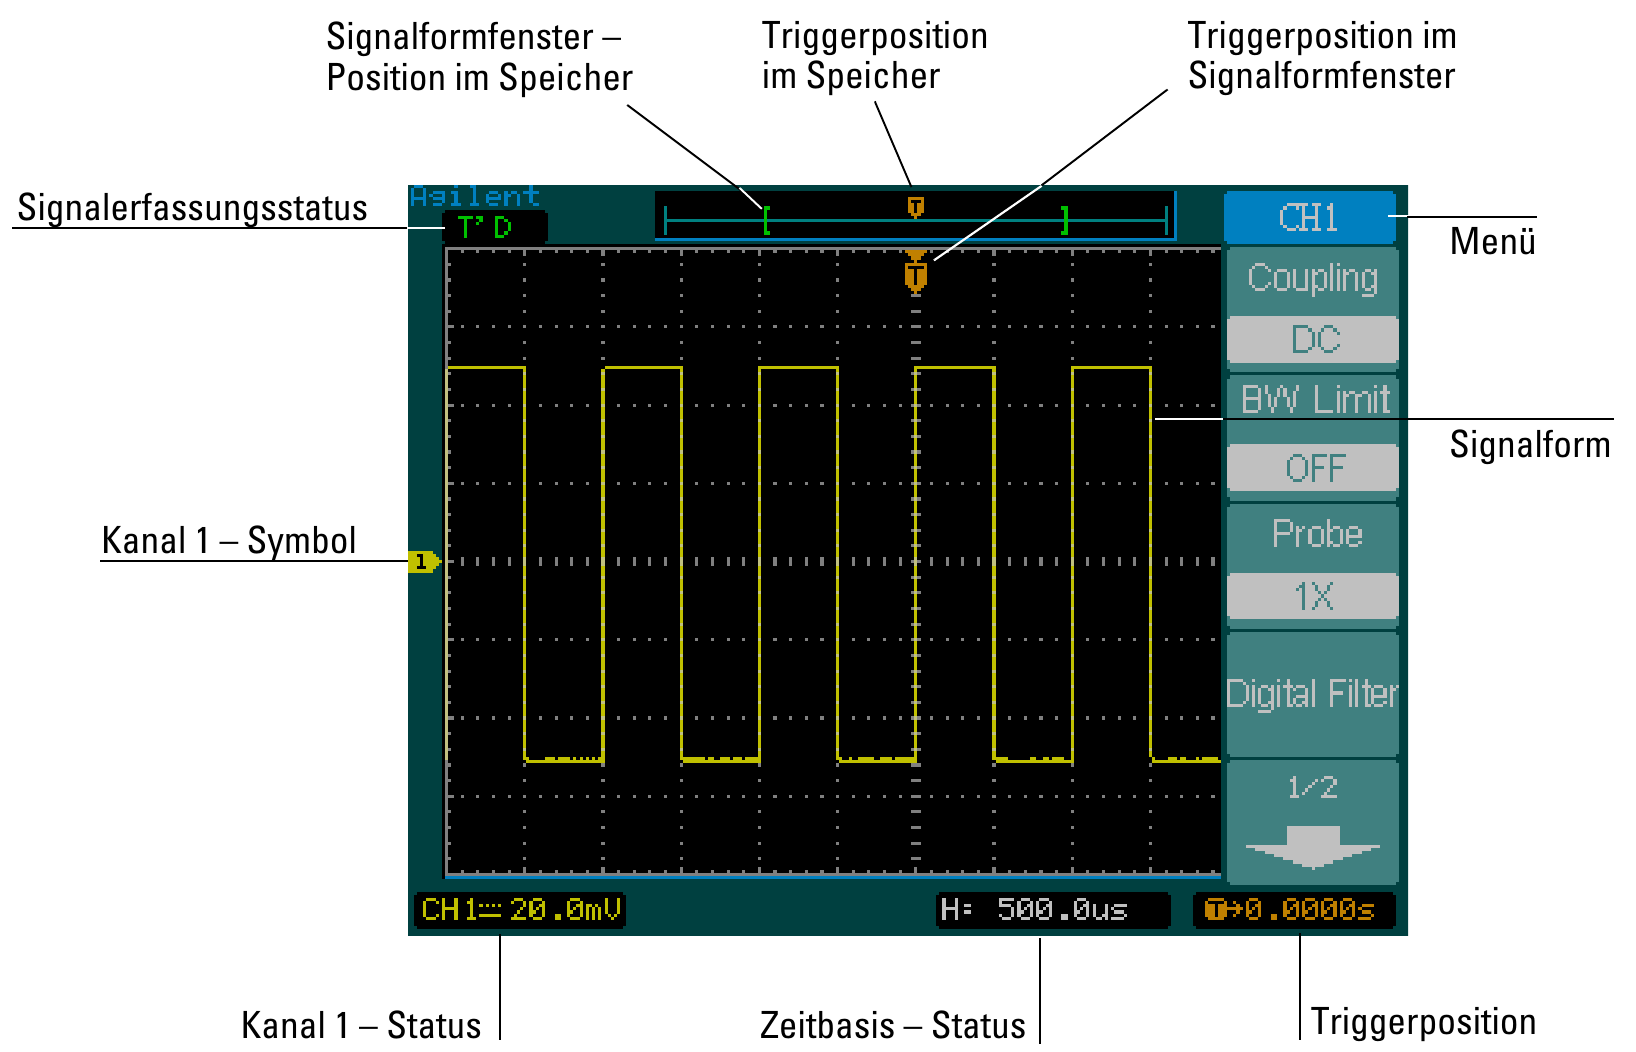
\includegraphics[scale=0.25]{Oszi/Bilder/oszi_anzeige.png}
\caption{Anzeige des Digital-Oszilloskops AT DSO3062A}
\label{Anzeige_Oszi}
\end{figure}
 
Es ist wichtig die maximale Eingangsspannung am BNC-Anschluss eines Oszilloskops nicht zu überschreiten, um Schäden zu vermeiden. Die maximale Eingangsspannung des Digital-Oszilloskop Agilent Technologies DSO3062A liegt bei $300V$.

%---------------------------------------------------------

\subsection*{Messen einer Wechselspannung}

\begin{figure}[H]
\centering
\subfigure[Schaltungsaufbau]{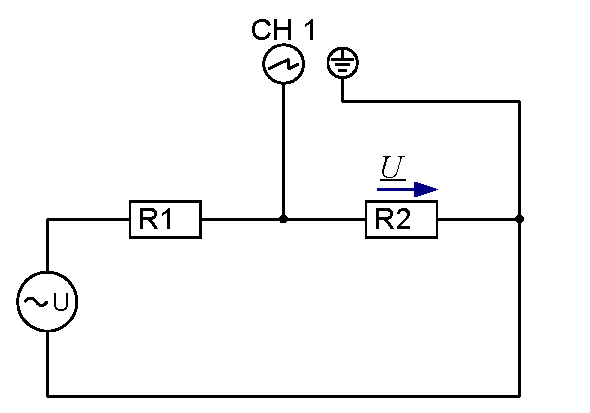
\includegraphics[scale=0.6]{Oszi/Bilder/oszi_AC.pdf}}
\subfigure[Anzeige des Oszilloskops]{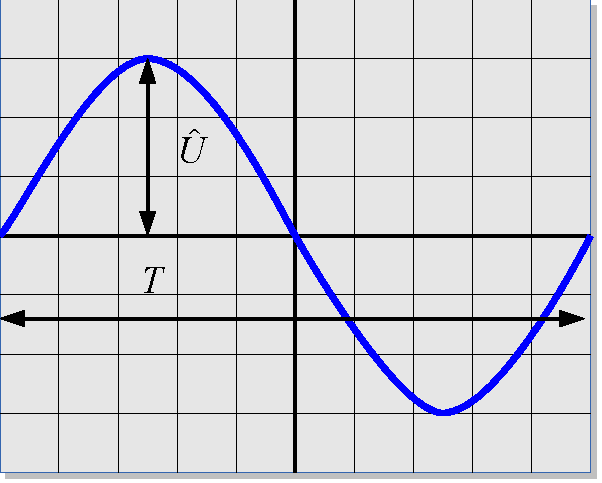
\includegraphics[scale=0.6]{Oszi/Bilder/oszi_AC_Anzeige.pdf}}
\subfigure[Beispiel  Spannung \underline{U}]{
\begin{minipage}[b]{5cm}
\begin{eqnarray*}
CH1  =			& 2V\\
\\
\hat{U} = 		& \dfrac{2V}{div} \cdot 3 div\\
 	    =		& 6V\\
 	    \\
\underline{U}=	& \dfrac{\hat{U}}{\sqrt{2}} 
 			=	& \dfrac{6V}{\sqrt{2}}\\
 		\approx	& 4,2V\\
\end{eqnarray*}
\end{minipage}
}
\subfigure[Beispiel Preiodendauer T und Frequenz f]{
\begin{minipage}[b]{5cm}
\begin{eqnarray*}
H           =	& 2ms\\
\\
T			=	& \dfrac{2ms}{div} \cdot 10div\\
			=	& 20ms\\
			\\
f			=	& \dfrac{1}{T}
			=	& \dfrac{1}{20ms}\\
			=	& 50Hz\\
\end{eqnarray*}
\end{minipage}
}
\caption{Messen einer Wechselspannung}
%\label{?}
\end{figure}

%-----------------------------------------------------------------------------
\newpage
\subsection*{Messen von Strömen}

Um den Strom mit Hilfe eines Oszilloskops zu ermitteln, wird die Spannung an einem bekannten Widerstand gemessen und mit Hilfe des ohmschen Gesetzes berechnet.

\begin{figure}[H]
\centering
\subfigure[Schaltunsgaufbau]{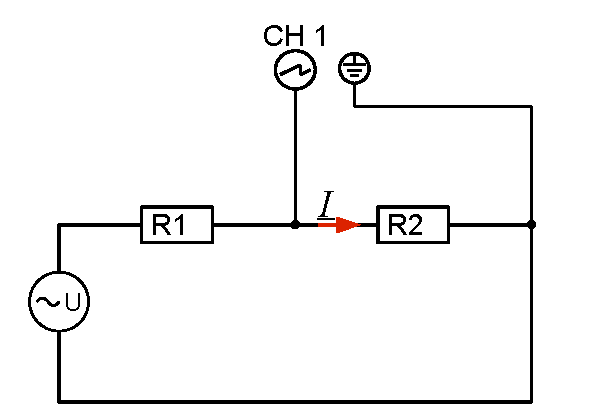
\includegraphics[scale=0.6]{Oszi/Bilder/oszi_ACI.pdf}}
\subfigure[Anzeige des Oszilloskops]{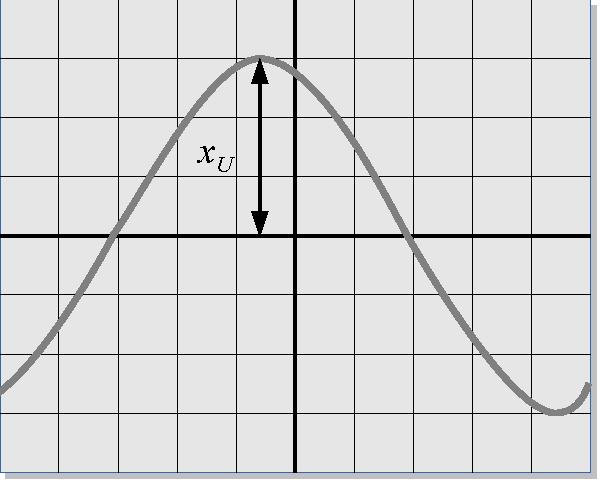
\includegraphics[scale=0.6]{Oszi/Bilder/oszi_ACI_Anzeige.pdf}}
\subfigure[Beispiel Spannung \underline{U}]{
\begin{minipage}[b]{5cm}
\begin{eqnarray*}
CH1		=		&	50mV\\
		\\
\hat{U} = 		& \dfrac{50mV}{div} \cdot 3 div\\
 	    =		& 0,15V\\
 	    \\
\underline{U}=	& \dfrac{\hat{U}}{\sqrt{2}} 
				= \dfrac{0,15V}{\sqrt{2}}\\
 		\approx	& 0,1V\\
\end{eqnarray*}
\end{minipage}
}
\subfigure[Beispiel Strom \underline{I}]{
\begin{minipage}[b]{5cm}
\begin{eqnarray*}
R2	 	=		& 1\Omega\\
		\\
\underline{I}  	= 		& \dfrac{U}{R} 
				= \dfrac{0,1V}{1\Omega}\\
		=		& 0,1A
\end{eqnarray*}
\\
\\
\\
\end{minipage}
}
\caption{Messen eines Wechselstroms}
\end{figure}

%-----------------------------------------------------------------------------
\newpage
\section*{Versuch}

\subsection*{Messen von Spannungen}

\begin{enumerate}
\item Lege eine Wechselspannung von $50Hz$ und  $U_{pp} =10V$ an eine Reihenschaltung von zwei Widerständen. Ermittle mit Hilfe des Oszilloskops die Spannungsabfälle an den einzelnen Widerständen und Ermittele den Strom der durch die beiden Widerstände fließt.
\item Ermittele mit Hilfe eines ohmschen Widerstandes, dessen Größe bekannt ist, den Widerstandswert der Blackbox. Überprüfe das Ergebnis mit Hilfe eines Widerstandsmessgerätes.
\item Nimm die Resonanzkurve des Stromes $\underline{I}$ und der Gesamtimpedanz $\underline{Z}$ des Reihenschwingkreises auf (siehe Abbildung \ref{resonanz}). Verwende hierfür einen Eingangsfrequenzbereich von $1kHz$ bis $1MHz$. Nimm mindestens 15 Messwerte auf und zeichne den Verlauf. Achte darauf, dass die Eingangsspannung konstant $U_{pp} =10V$ ist. Der interessanteste Bereich der Resonanzkurve befindet sich in der Nähe der Resonanzfrequenz. Überlege dir vor Beginn der Messung, welche Frequenzpunkte du messen willst.
\item \emph{\textbf{Zusatzaufgabe:}} Überlegen Sie sich eine Möglichkeit die Wirkleistung messtechnisch zu ermitteln. Nehmen Sie 6 Messwerte im Eingangsfrequenzbereich von $1kHz$ bis $1MHz$ auf und prüfen Sie ihre Ergebnisse rechnerisch mit den Messwerten aus der vorherigen Aufgabe.
\end{enumerate}

\begin{figure}[H]
\centering
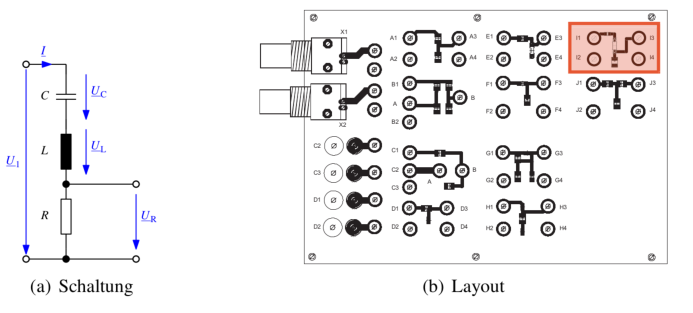
\includegraphics[scale=1]{Oszi/Bilder/resonanz}
\caption{Reihenschwingkreis: $C=10nF$, $L=470\mu H$, $R=50\Omega$}
\label{resonanz}
\end{figure}



